\documentclass[11pt]{article}
\ifdefined\PublicVersion
\usepackage[preprint]{acl}
\else
\usepackage[review]{acl}
\fi
\usepackage{times}
\usepackage{latexsym}
\usepackage[T1]{fontenc}
\usepackage[utf8]{inputenc}
\usepackage{microtype}
\usepackage{inconsolata}
\usepackage{graphicx}
\usepackage{amsmath,amssymb}
\usepackage{booktabs,tabularx,array}
\usepackage{url}
\usepackage{placeins}
\title{When Do Hallucination Improvements Compose?\\A Survey of Detection, Evaluation, and Mitigation in LLMs}
\ifdefined\PublicVersion
\author{Xincheng Li \\ School of Computer Science, University of Auckland \\ Email: \texttt{xli798@aucklanduni.ac.nz}}
\newcommand{\SurveyMaterials}{The evidence records and supporting materials are available at \url{https://github.com/lixincheng-xcl/LLM-Hallucination-Survey}.}

\else
\author{Anonymous ACL submission}
\newcommand{\SurveyMaterials}{The accompanying materials provide the extraction protocol and source-linked evidence records.}
\fi
\newcommand{\figwide}[3]{\begin{figure*}[t]\centering\includegraphics[width=\textwidth]{figures/#1}\caption{#2}\label{#3}\end{figure*}}
\begin{document}
\maketitle
\begin{abstract}
Hallucinations undermine the reliable use of large language models (LLMs), motivating methods that detect errors, evaluate factuality, and intervene in generation. Yet improvements in these components do not automatically establish that a combined system produces more reliable, useful answers. This survey examines the compatibility of their evidence. We first distinguish world factuality from source faithfulness and organize detection and mitigation by the information they use and the stage at which they operate. We then review benchmark targets and conduct a source-linked documentary audit of representative methods. The comparison shows why reported safeguards must be interpreted at their tested scope: fact counts do not measure required information, separate verification prompts do not establish independent judgment, and component evaluations need not characterize errors after intervention. We synthesize these distinctions into compatibility conditions covering reference frames, information retention, feedback--evaluation dependence, and residual-error validation, with computational access as a practical constraint. Finally, we outline prospective tests for detector--intervention combinations and identify the limits of the available evidence. \SurveyMaterials
\end{abstract}
\begin{figure}[t]
\centering
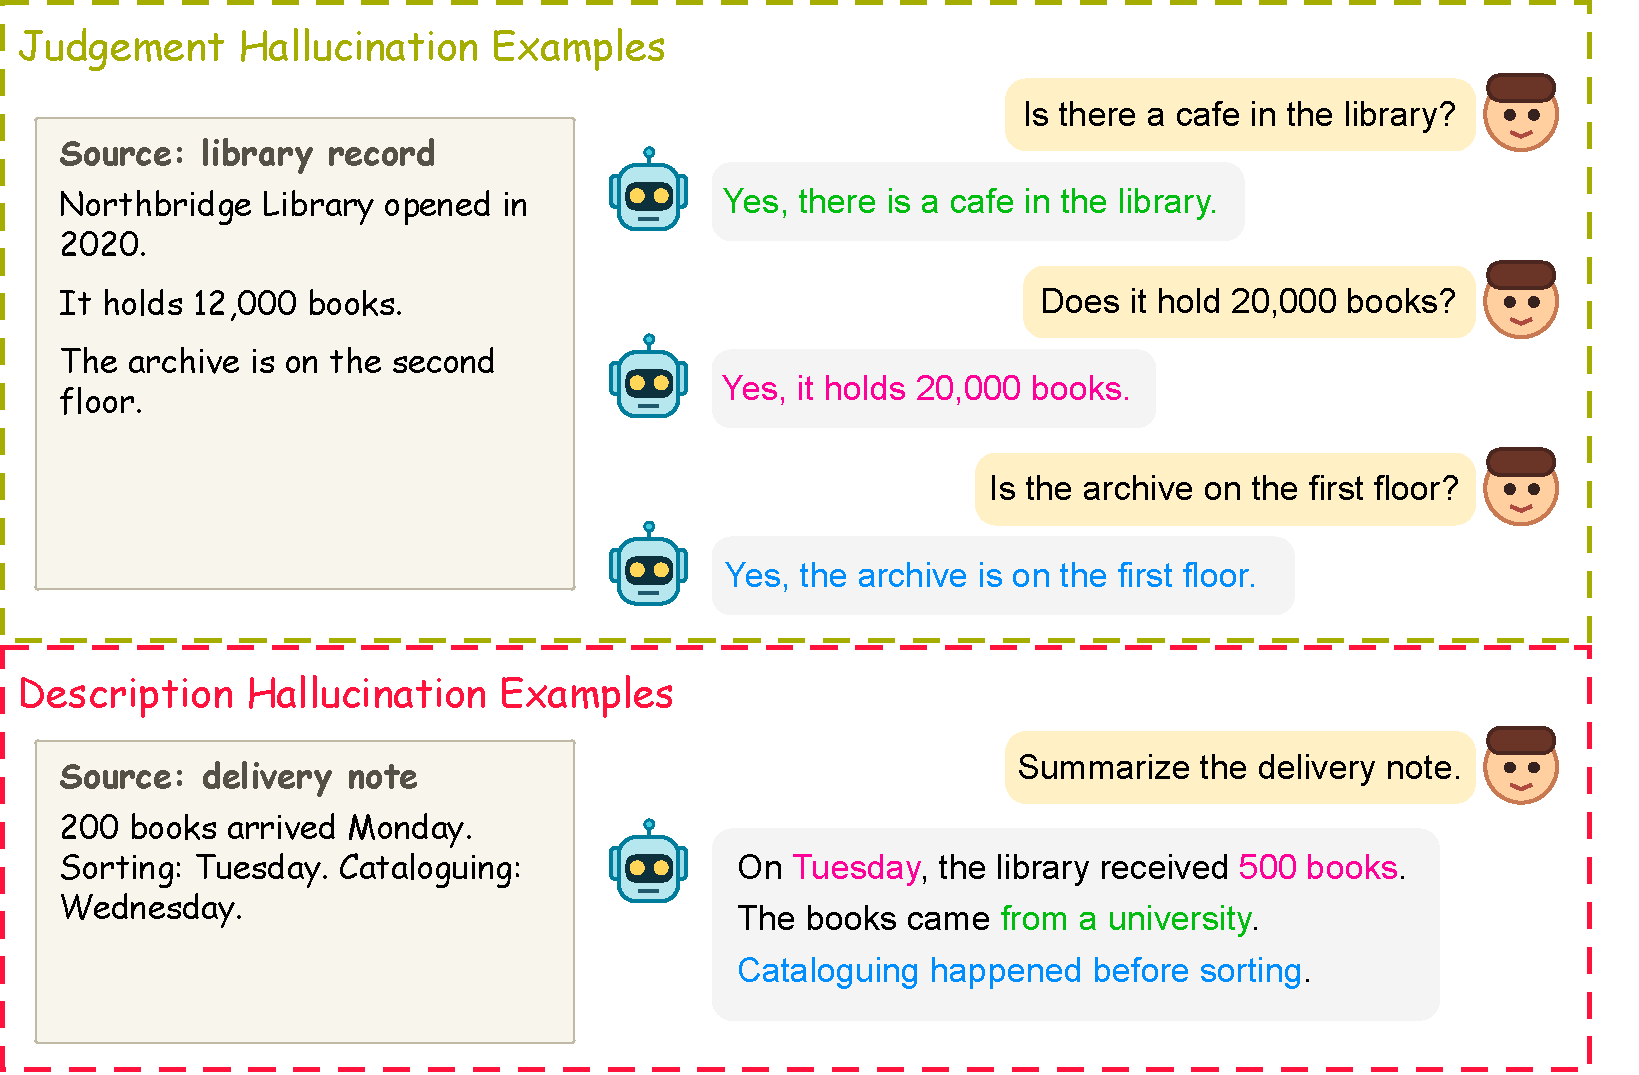
\includegraphics[width=\columnwidth]{figures/Fig1_hallucination_examples.pdf}
\caption{Illustrative hallucination examples in source-grounded question answering and summarization. Green, pink, and blue denote unsupported additions, attribute errors, and relation errors, respectively. Unsupported content is not necessarily false.}
\label{fig:examples}
\end{figure}
\section{Introduction}
A fluent answer from a large language model (LLM) is not necessarily justified. In question answering (QA), a model may repeat a misconception; in summarization, it may add a plausible detail absent from the source. Both are called hallucinations, although their correctness criteria differ: source-unsupported content can be factually correct \citep{lin-etal-2022-truthfulqa,cao-etal-2022-hallucinated}. Collapsing these settings obscures what a system improves.


In Figure~\ref{fig:examples}, the library record supports 12,000 books and a second-floor archive. The cafe assertion lacks support; the changed count and location contradict the record. The delivery summary also invents a university source and reverses events. Verification must specify the claim and its reference evidence.

Better hallucination detection and better generation are often treated as complementary safeguards. Their published results can nevertheless concern different reference evidence, answer populations, and information budgets. A detector evaluated on unrevised answers may encounter a different error distribution after correction. Likewise, a higher fraction of supported claims can coexist with fewer useful claims. The central question is therefore \emph{when evidence of a component improvement supports a claim about the combined system}.

We make three contributions. First, we connect reference frames, detection evidence, and intervention stages in a common comparison framework. Second, a bounded documentary audit records the tested safeguards and inference boundaries of representative methods, with primary-source locators. Third, we derive four compatibility conditions and a prospective reporting protocol from these comparisons. These are analytical contributions; we introduce no new detector or generation benchmark. Three questions organize the survey: \textbf{RQ1}, what reference defines an error; \textbf{RQ2}, what evidence supports a detector's use; and \textbf{RQ3}, when can detection and mitigation evidence support reliable, useful generation?

\figwide{Fig2_survey_structure.pdf}{The structure of this survey. Green boxes list representative studies for each branch.}{fig:structure}
\paragraph{Scope and organization.}
We cover text QA, long-form generation, summarization, dialogue, and retrieval-augmented generation (RAG), emphasizing ACL-family research and mechanism-defining work from other venues. Multimodal perception and general reasoning are excluded. Figure~\ref{fig:structure} maps concepts (\S\ref{sec:background}), detection (\S\ref{sec:detection}), evaluation (\S\ref{sec:evaluation}), mitigation (\S\ref{sec:mitigation}), and analysis (\S\ref{sec:analysis}).

\paragraph{Audit design.}
We fixed all thirteen named studies in an existing representative-method resource table before coding reporting properties. This purposive set spans source alignment, sampling, internal detection, training, retrieval, decoding, editing, revision, and abstention. For each primary full text, we inspected methods, evaluation, results, and relevant appendices, recording the reference frame, scoring unit, access, information control, feedback--evaluation separation, resources, and joint validation. A statement that evidence was not located is restricted to the inspected sections. All selected cases are retained; no field-wide frequency or pooled effect is inferred. Appendix~\ref{app:selection} and the accompanying codebook distinguish this audit from the broader contextual literature search and document reading depth.

\paragraph{Relation to prior surveys.}
\citet{Ji_2023} distinguish source faithfulness from world factuality across NLG tasks, while \citet{wang-etal-2024-factuality} organize LLM factuality evaluation and enhancement and identify obstacles to fair comparison. \citet{zhang-etal-2025-sirens} and \citet{Alansari_2026} analyze benchmarks, mitigation stages, evaluator limitations, and task-dependent trade-offs. \citet{schmidtova-etal-2025-eyes} audit human-evaluation reporting, including definitions, annotation procedures, and agreement. Building on these perspectives, our bounded audit examines how representative studies document the conditions needed to compare or combine detection and mitigation. Appendix~\ref{app:prior} records the inspected overlap and limits on novelty.


\section{Concepts and Scope}\label{sec:background}
\subsection{Reference frames}
\emph{World factuality} concerns agreement with externally established facts; \emph{source faithfulness} concerns support by supplied evidence. Neither entails the other: a response can repeat a false source faithfully or add a true but unlicensed detail \citep{cao-etal-2022-hallucinated,adlakha-etal-2024-evaluating}. BEGIN evaluates attribution in grounded dialogue under this distinction \citep{dziri-etal-2022-evaluating}.

Source-based labels should distinguish \emph{supported}, \emph{contradicted}, and \emph{not established}, retaining the last separately from world falsity. World verification additionally needs a specified evidence source, date, and unresolved-claim policy. These are operational choices, not a universal definition. HalluLens revisits definitions and benchmark construction \citep{bang-etal-2025-hallulens}; comparisons must map study-specific labels before comparing scores.

\subsection{Error relations and development}
Entity, attribute, and relation errors are orthogonal to reference frames: a wrong date can contradict either a document or a world fact. Annotation units also differ. ANAH provides sentence-level analysis, while HaluEval~2.0 extends empirical factuality analysis across domains \citep{ji-etal-2024-anah,li-etal-2024-dawn}.

Research moved from distinct task-specific correctness targets in 2022 toward atomic verification and black-box self-checking in 2023 \citep{min-etal-2023-factscore,manakul-etal-2023-selfcheckgpt}, followed by contextual monitoring and factuality alignment. Recent studies scrutinize judge reliability, information coverage, and temporal validity \citep{godbole-jia-2025-verify,samarinas-etal-2025-beyond,jiang-etal-2026-benchmarks}.

\figwide{Fig3_evaluation_taxonomy.pdf}{Taxonomy of hallucination evaluation methods for LLMs. The two branches distinguish generated-content evaluation from error-label prediction.}{fig:evaluation}
Three axes organize the comparison: reference frame, detection evidence, and intervention point. Benchmarks evaluate generated content or detectors; detectors can guide decoding. Fine-tuning and long-context studies motivate failures in supervision, knowledge access, and evidence use \citep{gekhman-etal-2024-fine,liu-etal-2024-lost}. Across axes, we compare evidence access, generator signals, supervision, and cost, separating decision criteria from deployment requirements.

\section{Detection: Evidence and Access}\label{sec:detection}
Detection estimates errors under a specified reference; Figure~\ref{fig:structure} groups methods by evidence and model access.

\subsection{External evidence}
Evidence-based methods compare outputs with supplied or retrieved knowledge. QAFactEval asks questions about summary content and checks answer recovery from the source; question generation and answerability affect its decisions \citep{fabbri-etal-2022-qafacteval}. AlignScore learns alignment across heterogeneous tasks and aggregates source-chunk/output-sentence scores \citep{zha-etal-2023-alignscore}. Both use trained auxiliaries; neither guarantees correct verification.

FActScore decomposes long answers into atomic facts and estimates their supported fraction relative to a designated source \citep{min-etal-2023-factscore}. VeriScore instead extracts verifiable claims, using surrounding context to resolve references \citep{song-etal-2024-veriscore}. Extraction changes the score denominator; missing support differs from contradiction. PrefixNLI extends entailment to incomplete prefixes, enabling feedback during decoding \citep{harary-etal-2026-prefixnli}.

\subsection{Sampling and consistency}
SelfCheckGPT scores a response sentence against additional responses to the same prompt \citep{manakul-etal-2023-selfcheckgpt}. Its NLI and prompting variants aggregate contradiction or non-support judgments across samples. This requires repeated generation rather than target-model probabilities; agreement can still reflect a repeated misconception.

Semantic uncertainty instead clusters sampled answers by semantic equivalence and estimates entropy over meanings, discounting paraphrase variation \citep{extsemanticuncertainty2023,extsemanticentropy2024}. Sentence-level QA uses mutual entailment; FactualBio relaxes this to non-contradiction with at least one-way entailment. The weighted estimator needs sequence probabilities; a discrete approximation uses cluster frequencies. SelfCheckGPT localizes inconsistency in a given response, whereas semantic entropy measures dispersion among answer meanings, targeting unstable confabulations. Both depend on sampling and comparison quality; stable false beliefs need not trigger either signal.

\subsection{Internal signals}
FOCUS combines token probabilities with attention-based uncertainty propagation from an accessible proxy model \citep{zhang-etal-2023-enhancing-uncertainty}. The target generator can remain black-box; the proxy must expose both signals. Hidden-state classifiers learn truth labels from activations \citep{azaria-mitchell-2023-internal}. Lookback Lens uses context-versus-generation attention features with a supervised linear classifier \citep{chuang-etal-2024-lookback}. Probes require representative training labels.

A separable activation pattern need not represent truth: associated falsehoods can resemble factual recall in controlled experiments \citep{cheang-etal-2026-llms}. Probes therefore need evaluation across natural error types and generators.

Source alignment cannot establish source truth; sampling and probes supply no independent factual evidence. ``Black-box'' and ``reference-free'' differ because access to generators, proxies, and verifiers must be specified separately.

\section{Benchmarks and Evaluation}\label{sec:evaluation}
\begin{table*}[t]
\centering\small
\setlength{\tabcolsep}{3pt}
\renewcommand{\arraystretch}{1.12}
\begin{tabularx}{\textwidth}{@{}p{.225\textwidth}p{.085\textwidth}p{.145\textwidth}p{.20\textwidth}X@{}}
\toprule
Benchmark & Setting & Size & Focus & Metrics \\
\midrule
TruthfulQA \citep{lin-etal-2022-truthfulqa} & Gen/MC & 817 questions (2022) & World factuality & Gen: truthfulness; informativeness; MC1 accuracy; MC2 true-answer mass \\
HaluEval \citep{li-etal-2023-halueval} & Dis & 35,000 samples & Mixed-task errors & Recognition accuracy \\
ANAH \citep{ji-etal-2024-anah} & Dis & $\sim$12k sentences & QA support; contradiction & Type accuracy; F1 \\
RAGTruth \citep{niu-etal-2024-ragtruth} & Dis & 17,790 responses & RAG faithfulness & Response/span P, R, F1 \\
ExpertQA \citep{malaviya-etal-2024-expertqa} & Gen & 2,177 questions & Correctness; attribution & Human factuality/support \\
TofuEval \citep{tang-etal-2024-tofueval} & Dis/Gen & 1,479 summaries* & Dialogue summaries & Balanced accuracy; error rate \\
HALoGEN \citep{ravichander-etal-2025-halogen} & Gen & 10,923 prompts & Domain factuality & Atomic hallucination rate \\
FaithBench \citep{bao-etal-2025-faithbench} & Dis/Gen & 750 summaries & Summary faithfulness & Balanced accuracy; macro F1; conditional error rate \\
FactBench \citep{fatahi-bayat-etal-2025-factbench} & Gen & 1,000 prompts & Verifiable claims & Hallucination score; precision \\
\bottomrule
\end{tabularx}
\par\smallskip\begin{minipage}{\textwidth}\footnotesize
* Paper-reported retained count; the source arithmetic is inconsistent. HALoGEN's count includes programming. FaithBench's selected cases are not a prevalence sample. Dis/Gen indicates distinct possible uses, not a shared metric.
\end{minipage}
\caption{Hallucination evaluation benchmarks for LLMs. `Dis', `Gen', and `MC' denote error-label discrimination, generated-content evaluation, and multiple choice, respectively; P and R denote precision and recall. Sizes count the stated units. Appendix~\ref{app:benchmarks} details the evaluation protocols.}
\label{tab:hallucination-benchmarks}
\end{table*}

Figure~\ref{fig:evaluation} separates generation evaluation from detector evaluation. World factuality and source faithfulness are reference frames for both; detector subbranches distinguish scoring units. Table~\ref{tab:hallucination-benchmarks} sizes count dataset units, not difficulty.

\subsection{Generation evaluation}
TruthfulQA evaluates misconception-oriented answers for truthfulness and informativeness, with a separate multiple-choice setting \citep{lin-etal-2022-truthfulqa}. ExpertQA distinguishes correctness from attribution through expert questions and claim-level judgments \citep{malaviya-etal-2024-expertqa}. HALoGEN uses domain-specific verifiers; FactBench combines user-derived prompts with web verification \citep{ravichander-etal-2025-halogen,fatahi-bayat-etal-2025-factbench}. Their scores are not interchangeable because evidence and verifier scopes differ.

TofuEval studies topic-focused dialogue summaries, where factuality must coexist with relevance and completeness \citep{tang-etal-2024-tofueval}. Precision needs coverage and refusal reporting, with explicit empty/unverifiable-answer policies.


Aggregation also changes the target. For $n>0$ extracted claims and $s$ supported claims, VeriScore combines $P=s/n$ with $R_K=\min(s/K,1)$ as $F_1@K=2PR_K/(P+R_K)$ for $s>0$, and zero otherwise \citep{song-etal-2024-veriscore}. Its domain-specific $K>0$ is the median extracted-claim count across evaluated responses. Unlike FActScore's basic support fraction, this rewards supported-claim quantity as well as precision. However, $R_K$ is not coverage of the information required by a question: extra supported details can raise it while leaving important aspects unanswered. Comparisons should fix $K$ and separately audit extraction, verification, and task-relevant coverage. FactBench's undecidable units additionally require an explicit aggregation policy \citep{fatahi-bayat-etal-2025-factbench}.

\subsection{Detector evaluation}
HaluEval mixes generated task-specific examples with human-annotated general queries; recognition accuracy need not transfer to unselected errors \citep{li-etal-2023-halueval}. ANAH annotates sentence-level types, evidence, and corrections; RAGTruth adds naturally generated RAG responses with error spans \citep{ji-etal-2024-anah,niu-etal-2024-ragtruth}. Response classification and span localization are different tasks: finding one error does not locate every unsupported claim.


Table~\ref{tab:hallucination-benchmarks}'s corpora do not supply every detector input. On fixed RAGTruth outputs, alignment can use source--response pairs \citep{niu-etal-2024-ragtruth}. SelfCheckGPT additionally needs prompt-conditioned samples from a declared generator; Lookback Lens needs attention features and probe-training labels. Specify feature models and prefixes; regenerating answers changes the evaluated outputs. Sentence-to-token conversion adds localization assumptions. TofuEval's sentence and summary decisions also require separate assessment \citep{tang-etal-2024-tofueval}.

FaithBench selects cases by detector disagreement, so its error frequency is conditional on selection \citep{bao-etal-2025-faithbench}. TRIVIA+ tests long contexts and noisy supervision \citep{chen-etal-2026-rethinking-evaluation}. Accuracy weights classes by prevalence; balanced accuracy weights them equally. Precision/recall require a declared positive class; span F1 requires tokenization and matching rules. Fix thresholds on validation data and match splits, generators, and evidence. Similar evaluator accuracy can still conceal biased system-level estimates \citep{godbole-jia-2025-verify}. Independently audit useful generation after mitigation.

\section{Mitigation: Interventions and Assumptions}\label{sec:mitigation}

Figure~\ref{fig:mitigation} organizes interventions by generation stage; Table~\ref{tab:method-comparison} contrasts reported safeguards with their inference boundaries. Context-aware decoding (CAD) favors supplied evidence, whereas Astute RAG reconciles conflicting knowledge \citep{shi-etal-2024-trusting,wang-etal-2025-astute}. Adhering to a record and answering what is true can require different policies; missing, ignored, and unreliable evidence motivate different interventions.

\figwide{Fig4_causes_mitigation.pdf}{Potential causes and mitigation methods of hallucination in LLMs. Colors group stages of the generation pipeline; hybrid methods may span multiple stages.}{fig:mitigation}

\begin{table*}[t]
\centering\small
\setlength{\tabcolsep}{4pt}\renewcommand{\arraystretch}{1.05}
\begin{tabularx}{\textwidth}{@{}>{\raggedright\arraybackslash}p{.19\textwidth}>{\raggedright\arraybackslash}p{.42\textwidth}>{\raggedright\arraybackslash}X@{}}
\toprule
Case / source location & Reported safeguard or experiment & Boundary for comparison or composition \\\midrule
FActScore, \S3.1, Tables 1/5, App. C & Support relative to a specified knowledge source; responding fraction and fact counts; editing using human factuality labels. & Information quantity is reported. Oracle-label editing does not validate the automatic estimator--editor combination. \\
CoVe, \S3.3 / Table 3 & Biographical FActScore and fact quantity are reported together; factored verification answers are generated without the original draft. & Precision and retained content can change together. Prompt separation does not establish independent factual knowledge. \\
Self-RAG, App. C.2 & Human checks of outputs and reflection tokens on 50 examples; support/plausibility excludes self-predicted irrelevant/no-support cases. & Human checks supplement self-scoring, but the conditional support/plausibility estimate does not characterize all outputs. \\
DoLa, Table 1 / \S4.2 / Apps. E--F & Truthfulness and informativeness; latency measurements under a specified device, batch, and generation length. & Measured overhead applies to that setup; it is not an equal-budget ranking against retrieval or revision methods. \\
SEAL, \S6 / App. E & A separate rejection experiment complements generation tests; tested beam settings differ from greedy baselines. & Generation factuality, selective answering, and compute allocation must be distinguished. \\
CRITIC, App. D & Detection metrics on initial answers and human analysis complement tool-assisted correction results. & These component analyses do not by themselves quantify fixed-detector calibration on revised errors. \\
\bottomrule
\end{tabularx}
\caption{Contrasts from the documentary audit. Locations refer to the cited primary papers discussed in Sections~\ref{sec:mitigation}--\ref{sec:analysis}; the supplementary records retain all thirteen cases. A boundary restricts the inference drawn here, not the validity of the original study.}
\label{tab:method-comparison}
\end{table*}


\subsection{Training and alignment}

FaithDial supplies curated source-grounded dialogue revisions for generation and critic supervision \citep{dziri-etal-2022-faithdial}. Self-Alignment improves self-evaluation through Self-Knowledge Tuning, ranks candidate responses by factuality, and forms response-level preference pairs for direct preference optimization (DPO) \citep{zhang-etal-2024-self}. For long answers, atomic-claim scores are averaged before ranking, so training preferences remain response-level.

FactAlign combines response-level Kahneman--Tversky optimization (KTO) with sentence-level fine-grained KTO (fKTO) \citep{huang-chen-2024-factalign}. Each sentence is treated as a continuation conditioned on the prompt and preceding sentences; binary factuality labels derive from support against retrieved Wikipedia evidence. Unlike DPO, fKTO needs no sentence-level preference pairs. UAlign incorporates confidence and semantic entropy into a reward model before proximal policy optimization (PPO) alignment \citep{xue-etal-2025-ualign}. RHIO targets contextual faithfulness: masking retrieval heads produces negative examples, control tokens distinguish faithful from unfaithful continuations, and contrastive decoding subsequently separates them \citep{huang-etal-2025-improving}. Finer feedback still inherits supervision errors.

\subsection{Retrieval and prompting}

FLARE retrieves actively when provisional continuations signal uncertainty, while context-faithful prompting changes instructions without retraining \citep{jiang-etal-2023-active,zhou-etal-2023-context}. Retrieval adds information but introduces selection errors and evidence conflicts. Self-RAG trains retrieval and reflection tokens that control when to retrieve and assess relevance, support, and utility; candidate continuations can then be ranked using these signals \citep{extselfrag2024}. Astute RAG instead uses a training-free, source-aware consolidation procedure: it elicits internal knowledge, compares it with retrieved passages, and iteratively resolves conflicts \citep{wang-etal-2025-astute}. Its reliability judgments remain fallible. These methods require separate audits of retrieval, conflict resolution, and evidence use.

\subsection{Decoding and internal intervention}

CAD amplifies the difference between context-conditioned and context-free token distributions \citep{shi-etal-2024-trusting}. For model parameters $\theta$, next token $y_t$, context $c$, query $x$, prefix $y_{<t}$, and contrast strength $\alpha\geq0$,

\begin{equation}\label{eq:cad}
p_{\mathrm{CAD}}(y_t)\propto\frac{p_\theta(y_t\mid c,x,y_{<t})^{1+\alpha}}{p_\theta(y_t\mid x,y_{<t})^\alpha}.
\end{equation}

CAD favors tokens whose probability increases when context is supplied, assuming that context deserves greater weight. DoLa instead subtracts earlier-layer from mature-layer log probabilities within a plausible-token set, dynamically selecting an earlier candidate layer by maximum Jensen--Shannon divergence from the mature layer \citep{extdola2024}. It assumes layerwise changes reveal useful parametric knowledge. Both reshape token distributions without independently checking truth.

TruthX learns separate semantic and truth-related latent spaces and edits internal representations along a learned direction \citep{zhang-etal-2024-truthx}. Lookback Lens trains a classifier over context-versus-generation attention ratios and selects candidate continuations with that classifier \citep{chuang-etal-2024-lookback}. Its mitigation closes the detector--generator loop, but also inherits detector errors. Such steering does not establish universal truth representations; architectural transfer needs testing.

\subsection{Revision and abstention}

Chain-of-Verification (CoVe) drafts an answer, generates verification questions, and revises the draft; its factored variants answer verification questions without the original draft \citep{dhuliawala-etal-2024-chain}. Separating verification from the draft reduces answer contamination, but all stages can still share a parametric misconception. CRITIC adds tool feedback before revision, providing an external correction signal \citep{extcritic2024}. WikiChat also grounds dialogue through retrieval and verification, coordinating these operations \citep{semnani-etal-2023-wikichat}. External feedback remains limited by search and tool reliability.

SEAL learns a rejection token and uses its probability to penalize uncertain decoding trajectories; the main experiments prohibit emitting that token, while a separate extension enables refusal \citep{huang-etal-2025-alleviating}. Refusal and revision need coverage and information retention alongside precision.

\section{Analysis and Future Directions}\label{sec:analysis}
The audit in Table~\ref{tab:method-comparison} yields four compatibility conditions. They are requirements for interpreting combined evidence, not a new scalar metric. We distinguish reported safeguards from stronger conclusions that those safeguards do not establish.

\paragraph{C1: Align the reference frame and evaluated population.}
FActScore operationalizes factual precision as support relative to a designated knowledge source, not unqualified world truth \citep[\S3.1]{min-etal-2023-factscore}. CAD strengthens use of supplied context \citep{shi-etal-2024-trusting}; DoLa and TruthX target truthfulness using internal signals \citep{extdola2024,zhang-etal-2024-truthx}. A faithful answer to a false document can therefore satisfy one target and violate another. Similarly, AlignScore's source alignment, SelfCheckGPT's sampled consistency, and semantic entropy's meaning dispersion observe different evidence \citep{zha-etal-2023-alignscore,manakul-etal-2023-selfcheckgpt,extsemanticentropy2024}. They cannot be ranked by treating all reported scores as interchangeable hallucination rates. A defensible comparison fixes the intended reference, the answer unit, and the evidence/unknown policy before matching metrics. Evaluation on selected disagreements or accepted answers must retain its conditional denominator.

\paragraph{C2: Preserve the information needed by the task.}
The audit does not support a blanket claim that methods ignore information retention. FActScore reports responding fractions and facts per response; DoLa reports truthfulness together with informativeness. Semantic entropy explicitly evaluates selective prediction through rejection-accuracy curves over retained-prediction fractions and their area (AURAC) \citep{extsemanticentropy2024}. CoVe reports both factual precision and fact quantity: in its Llama 65B biography experiment, factor+revise increases FActScore from 55.9 to 71.4 over few-shot prompting while the mean number of facts decreases from 16.6 to 12.3 \citep[Table 3]{dhuliawala-etal-2024-chain}. This documents a change in both dimensions; it does not isolate a causal length effect or establish lost task-relevant information.

The distinction is between \emph{reporting a safeguard} and \emph{controlling the desired quantity}. Fact counts, answer informativeness, and the fraction of questions answered are not required-aspect coverage. ICAT's aspect-based evaluation and studies of response length sharpen this distinction \citep{samarinas-etal-2025-beyond,zhao-etal-2025-response}. SEAL further separates ordinary generation with rejection-aware decoding from an explicit rejection experiment \citep[\S6]{huang-etal-2025-alleviating}. A comparison should report useful supported content and refusals, then compare risk at matched answered-question coverage where selection is involved.

\paragraph{C3: Trace feedback--evaluation dependence.}
Independence has several meanings. CoVe separates verification answers from the initial draft, reducing draft contamination without introducing independent knowledge. FactAlign trains with source-derived factuality labels, while Self-RAG learns reflection judgments used in generation \citep{huang-chen-2024-factalign,extselfrag2024}. Their evaluation must therefore be interpreted in relation to the feedback mechanism, not labeled independent merely because a separate stage or prompt exists.

Self-RAG provides a useful positive example and a boundary: Appendix C.2 reports human assessment of outputs and reflection tokens on 50 examples, but its support-and-plausibility assessment excludes cases predicted irrelevant or unsupported. Its support-and-plausibility estimate is conditional, rather than an all-output estimate. Lookback Lens uses GPT-4o for training labels and part of final judging, alongside human checks on XSum and NQ \citep[App. B]{chuang-etal-2024-lookback}; the audit retains both the shared component and the additional verification. Evaluator accuracy alone can also hide class-specific bias in system-level scores \citep{godbole-jia-2025-verify}. Final assessment should disclose shared models, evidence, labels, and selection rules and audit both high- and low-scoring outputs.

\paragraph{C4: Validate the detector on errors after intervention.}
A component test is informative without being a complete composition test. FActScore's Appendix C editing experiment uses human factuality labels, deliberately isolating estimator errors \citep{min-etal-2023-factscore}. CRITIC reports initial-answer detection and human error analysis alongside correction results \citep[App. D]{extcritic2024}. Lookback Lens explicitly uses its learned detector to select continuations \citep{chuang-etal-2024-lookback}. These are distinct designs; none should be collapsed into a binary claim that joint analysis is absent or sufficient.

A remaining question is whether a detector's operating point transfers to the residual errors produced by an intervention. Reasoning prompts can change both error frequency and detection cues \citep{cheng-etal-2025-chain}; consistent falsehoods can evade sampling-based signals \citep{extsemanticentropy2024,cheang-etal-2026-llms}. For erroneous candidate $E$, release decision $R$, and $P(E)>0$, the elementary identity
\begin{equation}\label{eq:release}
P(E\cap R)=P(E)P(R\mid E)
\end{equation}
shows why reducing candidate error alone does not guarantee fewer erroneous releases. It assumes no independence and is not itself a new theoretical result. Prospective tests should compare baseline, detector-only, mitigation-only, and combined systems on fixed questions, report erroneous releases per query, conditional error among released answers, and coverage, and recalibrate only on held-out validation data.

\paragraph{Resource compatibility is an additional constraint.}
Reported costs are not uniformly absent. DoLa measures latency in a fixed setup; SelfCheckGPT reports an API cost estimate. Such values cannot establish a hardware- and workload-independent ordering. Training-based FactAlign, retrieval-based Self-RAG, and iterative CoVe/CRITIC move expenditure between offline and online stages. SEAL's tested beam search and greedy baselines also use different decoding budgets. Report access requirements, training/annotation expenditure, generated tokens, retrieval/tool calls, and measured latency separately. Appendix~\ref{app:protocol} makes these conditions an unperformed prospective protocol, rather than presenting the audit as evidence of a new system's improvement.

\section{Conclusion}
\textbf{RQ1} requires a declared reference frame, claim unit, and unresolved-label policy. For \textbf{RQ2}, evidence access determines which errors a detector can identify, while reported safeguards must be read at their tested scope. For \textbf{RQ3}, the audited cases support four compatibility checks: align the correctness target, retain useful information, separate optimization from final judgment, and re-evaluate detection on post-intervention errors. The survey does not rank heterogeneous methods or establish a universal performance gain. It provides traceable comparisons and a prospective protocol for testing whether component improvements translate into more reliable useful generation.
\label{sec:mainend}
\section*{Limitations}
This is a critical narrative survey with a purposive documentary audit. The audit sample was fixed from an existing representative-method table before the new coding round; it is neither random nor an exhaustive sample of hallucination research. Its selection favors English text tasks and mechanism diversity. The broader discovery library and targeted update search have different reading depths from the audit; their records are not additional audited cases. Source-linked extraction is AI-assisted, not independent human double annotation. Ambiguous or unlocated evidence is retained as such. We report no agreement statistic, pooled effect estimate, model replication, or field-wide prevalence estimate. Heterogeneous tasks, evidence, judges, and budgets prevent a defensible global ranking. The compatibility conditions are a synthesis, not a validated predictive model; their operational benefit requires prospective testing. Figure~\ref{fig:structure} is a representative map rather than an exhaustive bibliography.
\section*{Ethical Considerations and AI Assistance}
Mischaracterizing a reliability safeguard as a guarantee can encourage unsafe deployment. We therefore distinguish original-study observations, our interpretation, and unperformed tests. The work analyzes public research documents and introduces no human-participant study or trained model. Full papers are linked rather than redistributed. Visual-design sources are credited in Appendix~\ref{app:selection}; illustrative interactions are synthetic. OpenAI Codex assisted literature retrieval, extraction, analysis, drafting, and artifact preparation. AI-assisted cross-checking does not constitute independent human verification. The evidence records expose source locations and uncertainties for author and reader inspection; responsibility for the submitted claims remains with the human author.
\clearpage
\bibliography{references,design_sources}
\clearpage
\appendix
\section{Selection, Provenance, and Reading Depth}\label{app:selection}
\subsection{Two evidence layers}
The contextual library supports a narrative account; the documentary audit supplies the comparative cases in Section~\ref{sec:analysis}. Their populations and reading depths must not be conflated. The audit includes AlignScore, FActScore, SelfCheckGPT, semantic entropy, Lookback Lens, FactAlign, Self-RAG, CAD, DoLa, TruthX, CoVe, CRITIC, and SEAL. These were all the named studies in a pre-existing resource table, chosen for mechanism diversity. The sample was fixed before the new extraction round on 5 October 2026; this is a recorded protocol, not an externally preregistered study.

We recorded primary publication URLs, PDF digests, inspected sections, and claim-specific locators. Extraction fields cover reference frame, scoring unit, evidence/access, information control, feedback--evaluation separation, resources, and joint validation. Information controls are described rather than collapsed into an adequate/inadequate score: fact quantity, task quality, required-aspect coverage, and answered-question coverage measure different things. Different prompts or model names do not prove statistically independent errors. A qualitative access requirement is not measured latency. ``Not located'' is bounded by the inspected source passages and is not proof of absence. The supplementary CSV preserves caveats for every case. Source checks and revisions were AI-assisted; no independent human annotation or inter-annotator agreement is claimed.

\subsection{Contextual discovery and targeted update}
The original contextual metadata snapshot is 15 September 2026. Discovery queried official ACL Anthology collections across ACL, EMNLP, NAACL, EACL, Findings, and TACL in 2022--2026. Twenty-five collections were available and five requested combinations unavailable. A broad title filter returned 1,766 records; three targeted additions and seven external studies brought the candidate pool to 1,776. The 87-study working library was selected for relevance, mechanism diversity, benchmark coverage, and counterevidence. Automatic title triage excluded 401 candidates; 1,288 remained unassessed reserve records. All selected titles and abstracts were screened; initial preparation inspected passages in fifteen papers, followed by claim-specific checks. These are workflow counts, not a full-text systematic-review flow.

The targeted update on 5 October 2026 checked closely related surveys and evaluation work against primary publication records. Its query and inclusion log is supplied separately; it does not purport to exhaust all intervening publications. Canonical published versions are preferred. The audit sample remains fixed, so update records and the broader bibliography do not increase its denominator. No model experiments, independent benchmark replications, or pooled effect estimates were performed.

\subsection{Visual provenance and coding examples}
The layouts of Figures~\ref{fig:examples}, \ref{fig:evaluation}, and~\ref{fig:mitigation} and Table~\ref{tab:hallucination-benchmarks} follow \citet{liu-etal-2024-lvlm-design}; Figure~\ref{fig:structure} follows \citet{liu-etal-2025-logical-design}. Their content addresses text LLMs. Figure~\ref{fig:examples} uses synthetic interactions. Figure~\ref{fig:mitigation} summarizes mechanisms proposed in the literature, not an experimentally identified causal decomposition. The figures provide a representative conceptual map; the source-linked audit adds protocol details that cannot be inferred from this map.

Detection branches are assigned by decision evidence, mitigation branches by the operation that changes generation. Thus Lookback Lens appears as attention-based detection and candidate-selection mitigation. RHIO combines training on induced negatives with contrastive decoding. Hybrid methods need not belong to exclusive categories. Source faithfulness is recorded separately from world factuality, and target-generator access separately from proxy or verifier access.

\subsection{Compatibility audit records}\label{app:audit}
The accompanying CSV contains one record per fixed case, with primary-source URLs, PDF digests, inspected sections, and locators for each substantive comparison. The records describe concrete reported controls rather than assign a universal quality score. They distinguish measured costs from access requirements, human labels from model judgments, and component analyses from tests of the complete detector--intervention system. Table~\ref{tab:method-comparison} highlights contrasts used in the main argument. Other selected studies remain in the record even when they do not support a simple positive or negative code. Tables~\ref{tab:audit-1}--\ref{tab:audit-3} summarize reported information controls and their boundaries.
\begin{table*}[tp]
\centering\small\setlength{\tabcolsep}{5pt}\renewcommand{\arraystretch}{1.12}
\begin{tabularx}{\textwidth}{@{}>{\raggedright\arraybackslash}p{.18\textwidth}>{\raggedright\arraybackslash}p{.42\textwidth}>{\raggedright\arraybackslash}X@{}}\toprule
Study & Reported information control & Interpretation boundary \\ \midrule
AlignScore \citep{zha-etal-2023-alignscore} & Fixed-output metric evaluation. Explicitly separates omission/content-selection errors from factual-consistency errors in PolyTope coding. A required-aspect-completeness or selective-answering outcome measure was not located in the inspected evaluation sections; omission exclusion is not such a measure. & Factuality and information selection are deliberately separated; detector performance does not alone establish usefulness after applying an output intervention. The altered PolyTope error definition and dataset overlap exclusions must be retained in comparisons. \\
FActScore \citep{min-etal-2023-factscore} & Reports responding fraction and fact quantity per response; explicitly warns that precision does not measure recall. The related editing experiment measures token preservation and agreement with human edits. Fact quantity and edit similarity are not required-aspect completeness. & Unsupported includes source absence as well as contradiction. Responding fraction and fact counts partly expose selective/short responses but cannot establish complete answers. Oracle-label editor results must not be attributed to the automatic estimator. \\
SelfCheckGPT \citep{manakul-etal-2023-selfcheckgpt} & Fixed-output detection/ranking on generated biographies. Descriptive token/sentence statistics are reported, but matched answered-question retention or required-aspect-completeness evaluation was not located in inspected \S{}\S{}6--7 and Appendix D. & Sample consistency can miss stable incorrect beliefs; the observed task is a selected GPT-3 biography set. Sentence PR-AUC and passage correlation do not measure correctness/completeness after editing or abstention. \\
Semantic entropy \citep{extsemanticentropy2024} & Explicit answered-question retention through rejection-accuracy curves and AURAC; FactualBio also evaluates retained fact predictions. This controls a retained-unit fraction, not required-aspect completeness of long answers. Biography question generation attempts to cover claim aspects but has acknowledged misses. & QA labels operationalize reference-answer agreement, not independently established world truth; SI explicitly preserves that target when a reference is wrong. FactualBio has only 21 biographies/150 claims. Retained-unit coverage differs from semantic completeness; systematic low-entropy errors remain outside the targeted confabulation mechanism. \\
Lookback Lens \citep{chuang-etal-2024-lookback} & Reports a general task-quality proxy (original MT-Bench score) alongside contextual-faithfulness score and NQ exact match. These do not establish matched required-aspect coverage or answer-completeness preservation for XSum. & The quality safeguard is task-specific and is not an equivalence test or matched-completeness study. Shared GPT-4o labeling/judging can preserve common errors despite human audit. Resource figures are approximate study-specific observations; transfer needs an auxiliary fitted head mapping. \\
\bottomrule\end{tabularx}
\caption{Documentary audit of reported controls (1/3). Descriptions retain original-study targets and unresolved reporting; precise passage locators and source digests are in the accompanying evidence records.}
\label{tab:audit-1}\end{table*}

\begin{table*}[tp]
\centering\small\setlength{\tabcolsep}{5pt}\renewcommand{\arraystretch}{1.12}
\begin{tabularx}{\textwidth}{@{}>{\raggedright\arraybackslash}p{.18\textwidth}>{\raggedright\arraybackslash}p{.42\textwidth}>{\raggedright\arraybackslash}X@{}}\toprule
Study & Reported information control & Interpretation boundary \\ \midrule
FactAlign \citep{huang-chen-2024-factalign} & Fact counts, factual precision and f1@K; literal Section 3.1 recall term is min(1, number of generated atomic statements/K), not a reference-aspect recall. MT-Bench provides helpfulness proxy. No matched answered-question coverage comparison located in inspected sections. & Corpus support is not universal truth. Generated fact quantity is not required-information completeness. For loss ablation compare the one-iteration full model with its ablation, not the three-iteration headline result. \\
Self-RAG \citep{extselfrag2024} & ASQA correctness, ROUGE, MAUVE and citation precision/recall; biography factual precision; ASQA maximum 100 generated tokens across baselines to limit length bias. Weight sweep exposes support-versus-fluency trade-off. These are not matched answered-question coverage or required-aspect completeness controls. & S\&P denominator is conditional on the model support/relevance decisions. Reflection agreement with GPT-4 is not independent truth adjudication. Citation recall concerns generated claims, not all information a user requires. \\
CAD \citep{shi-etal-2024-trusting} & Summarization reports ROUGE-L alongside FactKB and BERT-precision; QA reports exact match. Task quality is monitored, but neither reference-aspect completeness nor matched answered-question coverage is established. & NQ-Swap intentionally changes source entities, so success may require contradicting world knowledge. Do not classify its exact-match gain as world-truth improvement or infer a twofold latency from two distributions. \\
DoLa \citep{extdola2024} & TruthfulQA reports Truth, Info, their joint metric, and Reject; GPT-4 separately rates grammaticality/cohesiveness. These show informativeness/refusal trade-offs but are not matched coverage. For LLaMA-33B, Truth falls 62.5 to 56.4 while Info rises 69.0 to 92.4 and joint score rises 31.7 to 49.1. & Cannot add unlearned factual knowledge. Raw truth and informativeness may move in opposite directions. Latency result belongs to the reported hardware/output-length configuration. \\
\bottomrule\end{tabularx}
\caption{Documentary audit of reported controls (2/3). Descriptions retain original-study targets and unresolved reporting; precise passage locators and source digests are in the accompanying evidence records.}
\label{tab:audit-2}\end{table*}

\begin{table*}[tp]
\centering\small\setlength{\tabcolsep}{5pt}\renewcommand{\arraystretch}{1.12}
\begin{tabularx}{\textwidth}{@{}>{\raggedright\arraybackslash}p{.18\textwidth}>{\raggedright\arraybackslash}p{.42\textwidth}>{\raggedright\arraybackslash}X@{}}\toprule
Study & Reported information control & Interpretation boundary \\ \midrule
TruthX \citep{zhang-etal-2024-truthx} & Truth, Info, joint score and no-comment counts; original-model perplexity and cross-task accuracy supplement quality. They monitor refusal/informativeness, not matched answered coverage or required information completeness. & Two-fold in-domain validation and multiple-choice transfer do not establish general free-generation truth calibration. Editing cannot guarantee truth or inject missing knowledge (Limitations p.10). \\
CoVe \citep{dhuliawala-etal-2024-chain} & Correct/incorrect entity counts, multi-span precision/recall/F1, biography fact count with FActScore. Same-generator biography result 55.9 to 71.4 FActScore accompanies 16.6 to 12.3 facts. A separate Llama-2-chat clipping control is not a matched-length CoVe control. & Precision gain does not establish preservation of all correct or required facts. Closed-book checks remain bounded by model knowledge; shorter output is a measured trade-off, not proof of the entire gain being due to deletion. \\
CRITIC \citep{extcritic2024} & QA EM/F1 and qualitative/manual refusal and incorrect-correction categories; math answer correctness; toxicity task reports fluency/diversity proxies. No matched answered-question coverage or required-aspect preservation located. Non-oracle CRITIC and oracle CRITIC* must be kept separate. & Table 6 error-type percentages have a less explicit denominator than a full transition matrix; do not treat 10\% incorrect correction as the population rate. Oracle CRITIC* is not deployable verification; math/toxicity results do not directly measure factual hallucination. \\
SEAL \citep{huang-etal-2025-alleviating} & Biography correct-claim counts and FActScore; LongFact precision/R@48/F1@48; separate refusal experiment reports known-question accuracy versus unknown-question rejection across tau; instruction following is checked. R@48 uses truthful-fact count relative to 48, not required-aspect recall or matched question coverage. & Known/unknown status is a correctness/popularity proxy, not direct access to parametric knowledge. Main result cannot be interpreted as answer abstention. Biography sample count conflicts between Table 8 (138) and Appendix B.2 (183), unresolved. \\
\bottomrule\end{tabularx}
\caption{Documentary audit of reported controls (3/3). Descriptions retain original-study targets and unresolved reporting; precise passage locators and source digests are in the accompanying evidence records.}
\label{tab:audit-3}\end{table*}


\FloatBarrier

\subsection{Comparison with prior surveys}\label{app:prior}
The source-linked prior-survey record covers general NLG hallucination, LLM factuality, broad LLM hallucination, human-evaluation reporting, and detection/mitigation reviews. Its purpose is to delimit the contribution, not establish that a concept is absent from an entire literature. The resulting contribution claim is a cross-stage compatibility synthesis applied to a bounded sample. No first-survey or first-audit claim is made.


\section{Benchmark Units and Protocol Caveats}\label{app:benchmarks}
Table~\ref{tab:benchmark-caveats} supplies the counting and interpretation details behind Table~\ref{tab:hallucination-benchmarks}. A benchmark may support both a description of generated errors and evaluation of a detector, but those uses require different denominators and sampling assumptions. In particular, reporting error frequencies within deliberately selected difficult examples does not estimate a generator's error prevalence on ordinary requests.

\begin{table*}[tp]
\centering\small
\setlength{\tabcolsep}{5pt}\renewcommand{\arraystretch}{1.14}
\begin{tabularx}{\textwidth}{@{}p{.17\textwidth}X@{}}\toprule
Benchmark & Unit, protocol, and limitation \\\midrule
TruthfulQA & The original 2022 benchmark contains 817 questions. Generation measures truthfulness/informativeness; MC1 measures single-true accuracy, and MC2 normalized probability mass assigned to true answers. The \href{https://github.com/sylinrl/TruthfulQA}{official January 2025 update} introduced two-option choices and revised the question set. Report the dataset version and MC protocol separately; answer selection is not detector classification. \\
HaluEval & The 35,000 examples combine task-specific generated examples with a human-annotated general-query portion. Artificial and naturally generated errors should be reported separately rather than treated as one deployment distribution. \\
ANAH & Approximately 12,000 annotated sentences provide error types, evidence, and corrections. Generative versus discriminative annotators describe detector implementations; their task remains prediction of annotation labels. \\
RAGTruth & The 17,790 responses come from 2,965 prompts and six generators, not 17,790 independent documents. Response classification and span localization have different matching rules and must be evaluated separately. \\
ExpertQA & The 2,177 expert-curated questions support factuality and attribution analysis. Correctness and cited-source support are separate judgments; exact evaluation subsets and answer-generation conditions matter. \\
TofuEval & Section 3.3 reports 1,500 initial summaries, removal of 23, and 1,479 retained summaries. Those values are arithmetically inconsistent. We retain the reported 1,479 rather than invent a corrected dataset size. Topic relevance and completeness are separate from factual consistency. \\
HALoGEN & The 10,923 prompts cover all nine domains, including programming. That is the complete-suite count, not a verified text-only subset size. Different domain verifiers do not constitute one universal human truth oracle. \\
FaithBench & The 750 summaries derive from 75 passages and ten models, selected using detector disagreement. This supports difficult-case detector analysis; error frequencies are conditional on selection, not population prevalence. \\
FactBench & The 1,000-prompt snapshot uses user-derived prompts and fine-grained verification. Supported, unsupported, and undecidable units require explicit aggregation rules. A dynamic benchmark needs a fixed version for reproducible comparisons. \\
\bottomrule\end{tabularx}
\caption{Evaluation units, protocols, and limitations of the benchmarks in Table~\ref{tab:hallucination-benchmarks}.}
\label{tab:benchmark-caveats}
\end{table*}

\section{Supplementary Comparative Evidence}\label{app:comparisons}
Tables~\ref{tab:extra-evaluation}--\ref{tab:extra-mitigation} extend the main synthesis with complementary studies. The final column states the inference boundary used in this survey; it is not an assertion that the original authors omitted every proposed test. These studies expand coverage of mechanisms and failure conditions rather than form a ranked list. Descriptive entries are grounded in the recorded primary metadata and selected source passages, with reading depth retained in the repository.
\begin{table*}[tp]
\centering\small\setlength{\tabcolsep}{5pt}\renewcommand{\arraystretch}{1.18}
\begin{tabularx}{\textwidth}{@{}p{.22\textwidth}p{.34\textwidth}X@{}}\toprule
Study & Mechanism or evaluation design & Comparative implication and boundary \\\midrule
TRUE \citep{honovich-etal-2022-true-evaluating} & Standardizes factual-consistency datasets across tasks and evaluates metrics at the example level. & Instance discrimination differs from system-level correlation. Combined existing tasks do not estimate real-world hallucination prevalence. \\
AggreFact analysis \citep{tang-etal-2023-understanding} & Stratifies summarization error annotations by generating model and error type; metric gains vary across strata. & Pooled scores can hide weaknesses on newer generators or rare error types. \\
BUMP \citep{ma-etal-2023-bump} & Uses minimally differing human-written summary pairs with one introduced error. & A controlled error-sensitivity probe complements natural generation data; minimal pairs do not reproduce the full distribution of model errors. \\
ALCE \citep{gao-etal-2023-enabling} & Evaluates answer quality and citation quality in end-to-end retrieval and cited generation. & Citation presence, citation support, and factual correctness are distinct criteria. A plausible citation is not by itself evidence. \\
LongEval \citep{krishna-etal-2023-longeval} & Studies fine-grained human judgments and partial annotation for long summaries. & Fine-grained annotation requires agreement and coverage reporting; partial annotation does not exhaustively verify all claims. \\
FACTOR \citep{muhlgay-etal-2024-generating} & Transforms factual corpora into true versus false continuation choices. & Controlled factual choice evaluates a different task from open-ended generation and error localization. \\
ReEval \citep{yu-etal-2024-reeval} & Perturbs evidence to create dynamic tests of evidence use under retrieval. & Static accuracy may reflect memorized knowledge rather than source adherence; counterfactual evidence requires an explicit faithfulness target. \\
Core \citep{jiang-etal-2025-core} & Filters redundant or uninformative subclaims before factual precision aggregation. & Trivial repetitions can inflate precision; informativeness and coverage are complementary criteria. \\
TRIVIA+ \citep{chen-etal-2026-rethinking-evaluation} & Adds long-context RAG detection data and controlled sample-dependent label noise. & Long-context and noisy-label tests complement evaluation on clean labels. \\
RGB \citep{extrgb2024} & Separates noise robustness, negative rejection, information integration, and counterfactual robustness in English/Chinese RAG. & Retrieval conditions define distinct RAG abilities, not one interchangeable hallucination score. \\
\bottomrule\end{tabularx}
\caption{Additional benchmarks and evaluation protocols for hallucination in LLMs.}
\label{tab:extra-evaluation}
\end{table*}

\begin{table*}[tp]
\centering\small\setlength{\tabcolsep}{5pt}\renewcommand{\arraystretch}{1.18}
\begin{tabularx}{\textwidth}{@{}p{.22\textwidth}p{.34\textwidth}X@{}}\toprule
Study & Mechanism or evaluation design & Comparative implication and boundary \\\midrule
WeCheck \citep{wu-etal-2023-wecheck} & Aggregates weak labels over actual generated samples, then learns a noise-aware classifier. & Supervision quality and error distribution distinguish a learned consistency model from zero-shot entailment. \\
FactKB \citep{feng-etal-2023-factkb} & Uses knowledge-base factual pretraining with entity/relation objectives for factuality evaluation. & Structured supervision targets relation errors; broader transfer requires separate evidence. \\
TrueTeacher \citep{gekhman-etal-2023-trueteacher} & Uses LLM-labeled model-generated summaries to train a smaller consistency evaluator. & Distillation trades annotation cost for teacher-label dependence; generated errors differ from artificial perturbations. \\
FENICE \citep{scire-etal-2024-fenice} & Extracts atomic claims and aligns them to a source using natural language inference (NLI). & Local alignment improves interpretability, while claim extraction and entailment both remain possible error sources. \\
FactReasoner \citep{marinescu-etal-2025-factreasoner} & Models evidence--claim logical relationships probabilistically after decomposition/retrieval. & Joint reasoning differs from independently verifying claims; its result still depends on evidence retrieval and relation estimates. \\
Future context \citep{lee-etal-2026-enhancing} & Samples continuations and uses them as clues for black-box hallucination detection. & Generated continuations extend consistency checking without supplying independent external verification. \\
FaithLens \citep{si-etal-2026-faithlens} & Trains detection and explanations using filtered synthetic data, supervised fine-tuning (SFT), and rule-based reinforcement learning. & Explanation quality and decision accuracy require separate validation; fluency alone does not establish explanation faithfulness. \\
QASemConsistency \citep{cattan-etal-2026-localizing} & Decomposes claims into predicate--argument QA pairs for fine-grained support localization. & Semantic error localization supplies a finer target than response-level binary classification. \\
\bottomrule\end{tabularx}
\caption{Additional hallucination detection and explanation methods for LLMs.}
\label{tab:extra-detection}
\end{table*}

\begin{table*}[tp]
\centering\small\setlength{\tabcolsep}{5pt}\renewcommand{\arraystretch}{1.18}
\begin{tabularx}{\textwidth}{@{}p{.22\textwidth}p{.34\textwidth}X@{}}\toprule
Study & Mechanism or evaluation design & Comparative implication and boundary \\\midrule
Factual confidence \citep{mahaut-etal-2024-factual} & Compares confidence estimators and checks stability under meaning-preserving input changes. & Confidence can be unstable across paraphrases; access and supervision requirements differ. \\
New-knowledge fine-tuning \citep{gekhman-etal-2024-fine} & Controlled closed-book QA experiments vary the amount of unfamiliar factual information in SFT. & The findings motivate knowledge-aware supervision within the studied fine-tuning setup. \\
Known facts \citep{jiang-etal-2024-large} & Examines layer-wise prediction dynamics when questions about the same fact yield correct versus incorrect answers. & Errors can reflect knowledge access rather than absence; measured patterns do not prove universal causal mechanisms. \\
Lost in the Middle \citep{liu-etal-2024-lost} & Evaluates how position of relevant evidence affects long-context use. & Evidence being present is insufficient for reliable use; its tasks are not themselves a comprehensive hallucination taxonomy. \\
Hidden-state limits \citep{servedio-etal-2025-hidden} & Tests factuality encoding on more realistic, model-dependent generated data. & Accuracy on synthetic true/false facts does not establish probe generalization to target-model outputs. \\
Unfamiliar supervision \citep{kang-etal-2025-unfamiliar} & Relates hallucination response patterns to supervision of unfamiliar fine-tuning examples, including reward-model errors. & Factuality alignment depends on how unknowns and reward errors are labeled. \\
Illusion of Progress \citep{janiak-etal-2025-illusion} & Examines lexical-overlap labels and response-length heuristics in detector evaluation. & Semantic validation and simple baselines remain necessary; an LLM judge is not automatically a gold standard. \\
CoT obscures cues \citep{cheng-etal-2025-chain} & Measures how reasoning prompts shift hidden/probability signals and detector effectiveness. & A generation intervention shifts the detector's input distribution, making calibration transfer uncertain. \\
Hallucination tax \citep{song-etal-2025-hallucination} & Studies refusal degradation after reinforcement fine-tuning, primarily on unanswerable mathematics, with reported transfer to factual QA. & Evidence is not a universal result for every factual-generation task. \\
Source preferences \citep{schuster-etal-2026-whose} & Controlled synthetic-source study of source preferences and repetition in conflicting English evidence. & Frequency and source cues influence conflict resolution; synthetic-source preference is not proof of real-world source credibility. \\
\bottomrule\end{tabularx}
\caption{Studies of hallucination mechanisms and reliability in LLMs.}
\label{tab:extra-analysis}
\end{table*}

\begin{table*}[tp]
\centering\small\setlength{\tabcolsep}{5pt}\renewcommand{\arraystretch}{1.18}
\begin{tabularx}{\textwidth}{@{}p{.22\textwidth}p{.34\textwidth}X@{}}\toprule
Study & Mechanism or evaluation design & Comparative implication and boundary \\\midrule
FaithfulRAG \citep{zhang-etal-2025-faithfulrag} & Models fact-level conflicts between retrieved and parametric knowledge before response generation. & Explicit reconciliation complements source preference; source adherence and world correctness remain distinct. \\
CoCoA \citep{khandelwal-etal-2025-cocoa} & Adapts token-level decoding using confidence/context distribution differences. & Adaptive and fixed contrast differ in conflict sensitivity; low-conflict behavior also matters. \\
Context-DPO \citep{bi-etal-2025-context} & Constructs preferences from faithful versus stubborn responses under knowledge conflict. & A context-faithfulness objective differs from truthfulness with respect to external facts. \\
\bottomrule\end{tabularx}
\caption{Additional hallucination mitigation methods for LLMs.}
\label{tab:extra-mitigation}
\end{table*}


\FloatBarrier
\section{A Common Reporting Protocol}\label{app:protocol}
The following protocol is a synthesis of the comparisons in Sections~\ref{sec:detection}--\ref{sec:analysis}, not a benchmark run. It can be used to evaluate whether an intervention in Figure~\ref{fig:mitigation} solves the kind of error illustrated in Figure~\ref{fig:examples} under the target in Figure~\ref{fig:evaluation}.

\begin{table*}[tp]
\centering\small\setlength{\tabcolsep}{4pt}\renewcommand{\arraystretch}{1.14}
\begin{tabularx}{\textwidth}{@{}p{.17\textwidth}p{.24\textwidth}p{.25\textwidth}X@{}}\toprule
Family / example & Required access or supervision & Principal extra resource & Important boundary \\\midrule
Source alignment / AlignScore & Source and output text; trained auxiliary model & Verifier inference over chunks & Auxiliary-model errors and evidence truncation \\
Claim verification / FActScore & Claim extraction, knowledge source, retrieval and verifier & Search and per-claim checks & Retrieval failure differs from disproof \\
Self-checking / SelfCheckGPT & Repeated outputs; no generator internals & Additional generation and comparisons & Repeated falsehood can appear consistent \\
Semantic entropy & Samples and semantic equivalence; likelihoods for weighted estimation & Sampling and clustering & Estimator access differs by variant \\
Probe / Lookback Lens & Attention maps and labeled training spans & Feature extraction and probe inference & Supervised contextual proxy, not proof of truth \\
Factuality alignment / FactAlign & Generator training and sentence-level factual feedback & Verification plus optimization & Reward errors can be reinforced \\
Retrieval control / Self-RAG & Training, retrieval, reflection-token supervision & Training and retrieved candidates & Reflection judgments need auditing \\
Contrastive decoding / CAD & Context-conditioned and context-free logits & Extra distribution at decoding & Greater source adherence can amplify false evidence \\
Layer contrast / DoLa & Intermediate layer predictions & Layer-output computation & Parametric knowledge is not external evidence \\
Representation editing / TruthX & Hidden states and learned auxiliary components & Auxiliary learning and intervention & Transfer beyond training conditions is uncertain \\
Verification / CoVe, CRITIC & Model calls; CRITIC also needs tools & Verification and revision rounds & Isolated prompts are not independent knowledge \\
Selective generation / SEAL & Rejection-token training and regularized decoding & Training; altered answering behavior & Lower risk must be interpreted at matched coverage \\
\bottomrule\end{tabularx}
\caption{Access requirements and computational resources of representative methods. Resource descriptions are qualitative and do not imply measured cost rankings.}
\label{tab:access}
\end{table*}

\subsection{Fix the target before selecting a metric}
Specify whether the target is world correctness, source support, or both; the answer unit; and the treatment of unknown or unverifiable claims. Record the generator/version, prompts, retrieval corpus/date, evidence truncation, decoding parameters, and judge/version. Use the same evidence and question distribution across systems where possible. If a method changes retrieval, separate retrieval quality from generation conditional on the retrieved passages.

For a nonempty extracted claim set $C$ and fixed evidence $E$, a schematic support precision is
\begin{equation}
P_{\mathrm{support}}(C,E)=\frac{\sum_{c\in C}\mathbf{1}[E\models c]}{|C|}.
\end{equation}
This expression describes an aggregation principle, not the complete implementation of every factuality metric. Extraction determines the denominator; duplicate, trivial, subjective, and undecidable claims need explicit handling. An empty answer is not assigned perfect useful factuality by this definition. FActScore and VeriScore motivate claim-level analysis, while Core highlights the role of informative subclaims \citep{min-etal-2023-factscore,song-etal-2024-veriscore,jiang-etal-2025-core}.

\subsection{Separate detection, localization, and generation quality}
For binary detection, report class prevalence, confusion counts, precision/recall/F1, and balanced accuracy, $\tfrac12(\mathrm{TPR}+\mathrm{TNR})$, where appropriate. Fix thresholds on independent validation data. For spans, specify tokenization and exact versus overlap matching. For continuous scores, report discrimination and calibration separately; neither establishes the truth of an individual answer. Inspect false-positive and false-negative examples across error types, evidence lengths, and generator families.

For generation, pair factuality with unique supported content and required-aspect coverage. A source-faithful answer may still omit the answer to the question. Human auditing should sample both high- and low-scoring outputs, use explicit instructions, and report disagreement or adjudication. LongEval provides relevant human-evaluation guidance \citep{krishna-etal-2023-longeval}. Avoid pooling scalar scores whose claim extraction, evidence, or unknown-label policy differs.

\subsection{Measure selection and revision effects}
Let $A_\tau$ be the answers retained by threshold $\tau$ among $N$ questions, and let $e_i$ indicate an erroneous answer under the declared reference frame. For nonempty $A_\tau$, define
\begin{equation}
\begin{aligned}
\mathrm{Coverage}(\tau)&=\frac{|A_\tau|}{N},\\
\mathrm{Risk}(\tau)&=\frac{\sum_{i\in A_\tau}e_i}{|A_\tau|}.
\end{aligned}
\end{equation}
Comparing risk at matched coverage prevents a system from appearing universally better merely by refusing more questions. This response-level selective-evaluation definition is distinct from SEAL's token-level training objective. For revision, count corrected errors, newly introduced errors, retained supported claims, and required information lost. Measure both before and after revision on the same initial drafts.

\subsection{Audit independence, robustness, and cost}
A verifier used for training or candidate selection should not be the sole final judge. Use independently collected labels or an independently audited evaluator. Test natural errors from held-out generators, difficult consistent falsehoods, evidence conflicts, context permutations, paraphrases, and updated facts. Disaggregate performance rather than interpreting an average as proof of transfer. Verify with Caution and temporal benchmark analysis motivate independent error inspection and timestamped evidence \citep{godbole-jia-2025-verify,jiang-etal-2026-benchmarks}.

Table~\ref{tab:access} summarizes method access and deployment trade-offs. Report offline annotation and training costs separately from inference calls, sampled tokens, retrieval requests, tool invocations, latency, and memory. A black-box method can be expensive, while an internal method can be unavailable even if computationally economical. Do not infer a fixed latency multiplier from the number of model distributions or stages without measurement. Comparisons should either match budgets or present a quality--cost trade-off.

% Genuine citations printed in imported figures; registered for BibTeX.
\nocite{adlakha-etal-2024-evaluating,azaria-mitchell-2023-internal,bang-etal-2025-hallulens,bao-etal-2025-faithbench,cao-etal-2022-hallucinated,cheang-etal-2026-llms,chuang-etal-2024-lookback,cohen-etal-2023-lm,dhuliawala-etal-2024-chain,dziri-etal-2022-evaluating,dziri-etal-2022-faithdial,extcritic2024,extdola2024,extselfrag2024,extsemanticentropy2024,extsemanticuncertainty2023,fabbri-etal-2022-qafacteval,fan-etal-2026-refl,fatahi-bayat-etal-2025-factbench,feng-etal-2024-dont,gema-etal-2025-decore,godbole-jia-2025-verify,harary-etal-2026-prefixnli,huang-chen-2024-factalign,huang-etal-2025-alleviating,huang-etal-2025-improving,ji-etal-2024-anah,jiang-etal-2023-active,jiang-etal-2026-benchmarks,li-etal-2023-halueval,li-etal-2024-dawn,lin-etal-2022-truthfulqa,liu-etal-2024-universal,malaviya-etal-2024-expertqa,manakul-etal-2023-selfcheckgpt,min-etal-2023-factscore,niu-etal-2024-ragtruth,ravichander-etal-2025-halogen,samarinas-etal-2025-beyond,semnani-etal-2023-wikichat,shi-etal-2024-trusting,song-etal-2024-veriscore,tang-etal-2024-tofueval,wang-etal-2024-factuality,wang-etal-2025-astute,wu-etal-2024-synchronous,xue-etal-2025-ualign,zha-etal-2023-alignscore,zhang-etal-2023-enhancing-uncertainty,zhang-etal-2023-sac3,zhang-etal-2024-self,zhang-etal-2024-truthx,zhang-etal-2026-stable,zhao-etal-2025-response,zhou-etal-2023-context}


\end{document}
